%Note di Ingegneria del Software
%Sommario: Pattern e stili Architetturali

\cornell{Problema}{Accoppiamento (tra classi, componenti, \ldots)\\
Nel caso l'applicazione non sia creata facendo uso di una struttura organizzata, questa risulterà molto difficile da scalare.\\
Inoltre se un'applicazione non è ben organizzata, questa non risponderà bene ai cambiamenti, rallentando di molto gli aggiornamenti alle ultime tecnologie (debito tecnologico).
L'anti pattern dato dall'avere un insieme di moduli non organizzati viene detto \textit{Big Ball of Mud}.}

\cornell{Layered Architecture}{Solitamente usato per applicazioni molto piccole.\\
Le componenti sono organizzate "a strati", in modo orizzontale.\\
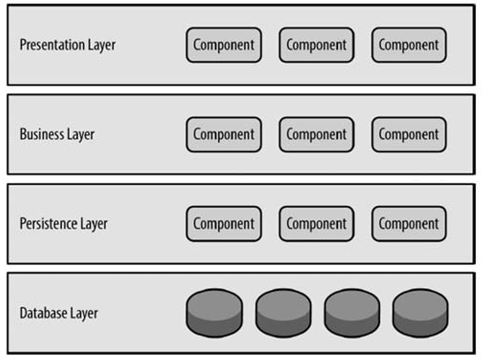
\includegraphics[scale=0.5]{images/65.png}}

\cornell{Caratteristiche della Layered Architecture}{L'architettura di questo tipo più comune è la cosiddetta \textit{3-tier architecture}, composta da Frontend, Business Logic e Persistenza.\\
Ogni strato ha una \textbf{singola} responsabilità.\\
Ogni strato parla solo con i layers adiacenti (imponendo quindi solo una dipendenza "verso il basso").\\
Le applicazioni sviluppate con questo stile sono semplici da testare, in quanto ogni layer può facilmente essere mockato.}

\cornell{Layers Chiusi vs Layers Aperti}{Prendiamo per esempio un'applicazione Layered, che sia composta da questi quattro strati:\\
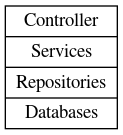
\includegraphics[scale=0.5]{images/66.png}\\
Nel caso si faccia una richiesta REST del tipo \texttt{GET professori/rcardin}, lo strato "services" fungerà solo da "passacarte".\\
In questo caso quindi si può adottare una struttura "a layer aperti", derogando ai principi layered classici e facendo in modo che il "controller" dialoghi direttamente con lo strato "repositories" (in questo caso si dice che il layer "services" è aperto).\\
Però: \begin{itemize}
\item È un approccio pericoloso
\item Introduce ulteriori dipendenze non controllate tra strati che non dovrebbero avere dipendenze
\item È un'eccezione che dovrebbe essere usata solo se il guadagno dato da questo è \textbf{Molto Alto} (Si suggerisce di mantenere il "least astonishment principle").
\end{itemize}}

\cornell{Considerazioni}{\begin{description}
\item [Buon Punto di Partenza] È un pattern general-purpose solido
\item [Architecture Sinkhole Anti-pattern] Si rischia di avere a che fare con un anti-pattern in cui gran parte delle richieste passano attraverso strati che fanno solo da "passacarte". In tal caso si consiglia di aprire alcuni layer.
\item [Scala male] In quanto tende a creare un'applicazione monolitica.
\end{description}}

\cornell{Analisi del Pattern}{\begin{tabularx}{\textwidth}{|c|c|X|}
                \hline
                \textbf{Agilità} & \cross & I piccoli cambiamenti sono isolabili, ma i grossi cambiamenti sono difficili a causa della natura monolitica del pattern.\\
                \hline
                \textbf{\makecell{Semplicità di\\ Installazione/Deploy}} & \cross & Difficile per grandi applicazioni a causa dei deployment monolitici.\\
                \hline
                \textbf{Testabilità} & \tick & Creare mock e stub dei layer è un'operazione semplice\\
                \hline
                \textbf{Performance} & \cross & Gran parte delle richieste attraversano molti layer, rallentando il sistema\\
                \hline
                \textbf{Scalabilità} & \cross & La Granularità troppo grossolana rende il sistema costoso da scalare.\\
                \hline
                \textbf{\makecell{Semplicità di\\Sviluppo}} & \tick & È un pattern ben conosciuto, solitamente ha connessione diretta con la compagnia che produce il software. \\
                \hline
        \end{tabularx}
}

\cornell{Architettura Event-Driven}{Un popolare pattern asincrono.\\
\begin{itemize}
\item È Molto adattabile
\item Produce applicazioni molto scalabili
\item I moduli di elaborazione degli eventi sono molto disaccoppiati ed hanno un obiettivo singolo
\item Gli eventi sono processari in modo asincrono
\end{itemize}\\
Esistono due topologie: \begin{itemize}
\item Mediator Topology
\item Broker Topology
\end{itemize}}

\cornell{Mediator Topology}{Vi sono tante componenti con pochissime responsabilità ciascuna che hanno vita propria (e che non sanno nulla l'uno degli altri)\\
L'evento generato viene inserito in un componente che sa quali altre componenti singole chiamare, ed in che ordine. Tale componente è detta \textbf{Mediator} (o anche Orchestrator)}

\cornell{Schema Esemplificativo}{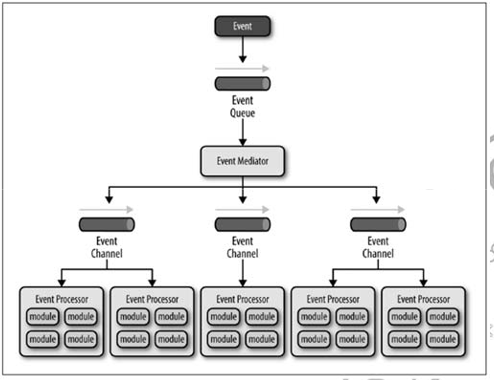
\includegraphics[scale=0.5]{images/67.png}}

\cornell{Mediator}{Il mediator \textbf{non effettua business logic} (trasformazioni, ad esempio.)\\
È fondamentale fare uso di un canale di comunicazione asincrono come: \begin{itemize}
\item Una coda FIFO
\item Un canale Topic (In cui si inserisce un messaggio e chiunque è in ascolto su tale topic può leggere)
\end{itemize}}

\cornell{Event Processor}{\begin{itemize}
\item Contiene la business Logic
\item È responsabile della pubblicazione di nuovi eventi
\end{itemize}}

\cornell{Broker Topology}{Non contiene alcun mediatore.\\
Ogni event processor legge un evento da un topic e pubblica un nuovo evento in un altro topic in modo diretto.\\
Il flusso per rispondere ad una richiesta è quindi distribuito.\\
Tramite questa topologia è semplice aggiungere moduli in ascolto sulle code, invece di andare a modificare il codice di un eventuale Mediator.}

\cornell{Schema Esemplificativo}{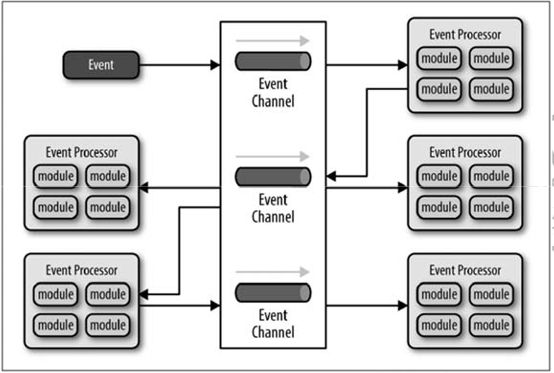
\includegraphics[scale=0.5]{images/68.png}}

\cornell{Considerazioni}{Le architetture ad eventi sono difficili da implementare. \begin{description}
                \item[È un'architettura completamente asincrona e distribuita] Con i conseguenti problemi che affliggono i sistemi distribuiti: remote process availability, lack of responsiveness e reconnection logic. In ogni caso qualiasi cosa potrebbe andare storto.
                \item[Mancanza di transazioni atomiche] Quali eventi possono essere avviati indipendentemente? Quale granularità mi è messa a disposizione per la loro gestione?
                \item[C'è bisogno di contratti forti per i processori di eventi] Come ad esempio un formato standard per la comunicazione dei dati, come JSON o XML.
\end{description}}

\cornell{Analisi}{\begin{tabularx}{\textwidth}{|c|c|X|}
                \hline
                \textbf{Agilità} & \tick & I cambiamenti sono generalmente isolati e sono fatti in modo veloce e con poco impatto sul sistema\\
                \hline
                \textbf{\makecell{Semplicità di\\ Installazione/Deploy}} & \tick & Il deploy è semplice, data la natura disaccoppiata delle componenti. La broker topology è quella più semplice da questo punto di vista.\\
                \hline
                \textbf{Testabilità} & \cross & Richiede client specializzati per il testing che siano in grado di generare eventi.\\
                \hline
                \textbf{Performance} & \tick & Alte performance, date le caratteristiche di asincronismo.\\
                \hline
                \textbf{Scalabilità} & \tick & Gli event processor sono scalabili separatamente, dando un controllo granulare sulla scalabilità\\
                \hline
                \textbf{\makecell{Semplicità di\\Sviluppo}} & \cross & La programmazione asincrona richiede contratti forti e gestione avanzata degli errori\\
                \hline
        \end{tabularx}
}

\cornell{Architettura A Microservizi}{Architettura ancora in fase di evoluzione.\\
Architettura fatta da tanti servizi, ogni servizio ha uno stack di persone dedicate alla gestione di tale servizio.\\
Il personale è quindi diviso in "Squad", in modo verticale (diversamente dal modo orizzontale dato dalle architetture layered)}

\cornell{Diagramma esemplificativo}{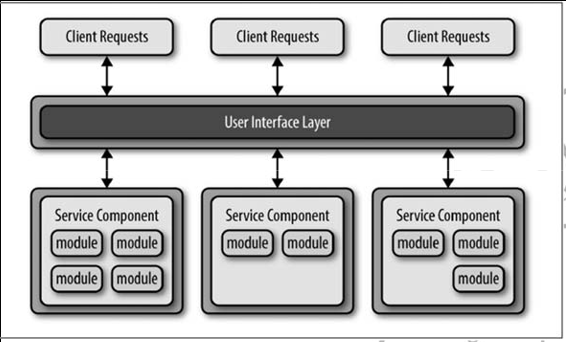
\includegraphics[scale=0.5]{images/69.png}}

\cornell{Problema}{Nell'architettura a microservizi si viene meno al principio DRY (Don't repeat Yourself), quindi si avrà replicazione di codice allo scopo di mantenere la separazione completa tra i microcontrollori}

\cornell{Topologia API-REST}{La più popolare.\\
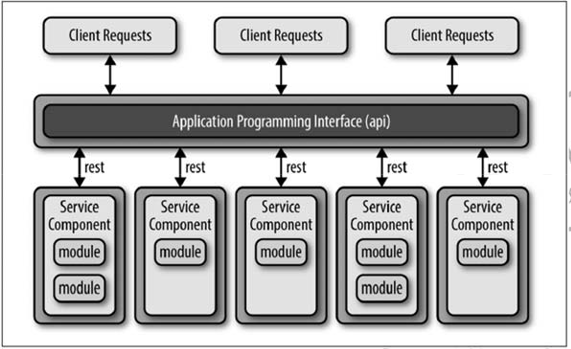
\includegraphics[scale=0.5]{images/70.png}\\
REST si mappa molto bene col protocollo HTTP, quindi posso esporre un URL e fare uso di chiamate REST per effettuare operazioni tramite delle API.}

\cornell{Topologia REST}{Si fa uso di chiamate REST per accedere ai microservizi.\\
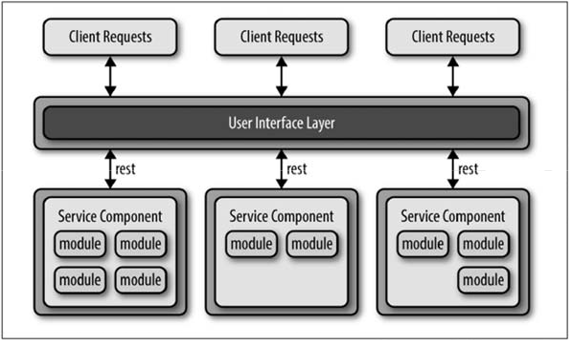
\includegraphics[scale=0.5]{images/71.png}}

\cornell{Centralized Message Topology}{Invece di esporre più endpoint, ho una rappresentazione unica di più microservizi.\\
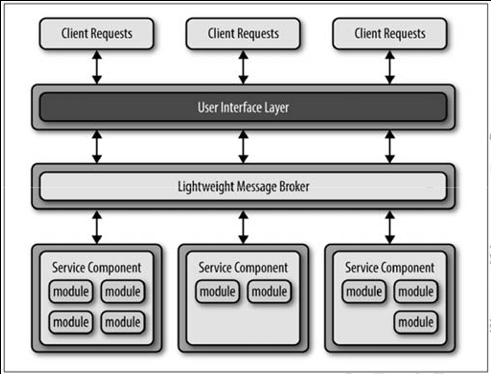
\includegraphics[scale=0.5]{images/72.png}}

\cornell{Analisi}{\begin{tabularx}{\textwidth}{|c|c|X|}
                \hline
                \textbf{Agilità} & \tick & Le modifiche sono solitamente isolate, il deploy è facile e veloce. L'accoppiamento è lasco.\\
                \hline
                \textbf{\makecell{Semplicità di\\ Installazione/Deploy}} & \tick & Il deploy è semplice a causa della natura disaccoppiata delle componenti. Hotdepoy e continuous delivery sono possibili.\\
                \hline
                \textbf{Testabilità} & \tick & Grazie all'isolamento delle funzioni di business, il testing può essere reso specifico. Le possibilità di avere una regressione sono basse.\\
                \hline
                \textbf{Performance} & \cross & Data la natura distribuita del pattern, le performance non sono proprio alte.\\
                \hline
                \textbf{Scalabilità} & \tick & I servizi sono scalabili separatamente. \\
                \hline
                \textbf{\makecell{Semplicità di\\Sviluppo}} & \tick & Lo scope di business è piccolo ed isolato, richiedendo quindi meno coordinazione tra i developers ed i team di development.\\
                \hline
        \end{tabularx}
}
